\chapter{Proper Distance, Kruskal Geometry, and Horizon Observers}

The Schwarzschild metric appears to become singular at the horizon.  The
curvature does not.  To separate those two statements, we first remove the
overall size of the black hole, then replace the radial coordinate by proper
distance from the horizon.  Near the horizon the resulting geometry is
ordinary flat spacetime written in accelerated coordinates.  Once that
geometry is drawn, questions about Alice, Bob, and Charlie become questions
about worldlines and light rays rather than verbal paradoxes.

\section{Scaling Out the Schwarzschild Radius}

Begin with primed coordinates so that the rescaled variables can later carry
the familiar names:
\begin{equation}
d\tau^2
=
\left(1-\frac{2MG}{r'}\right)dt'^2
-
\frac{dr'^2}{1-\frac{2MG}{r'}}
-
r'^2d\Omega_2^2.
\label{eq:l7-schwarzschild-dimensional}
\end{equation}
Introduce the Schwarzschild radius and dimensionless coordinates
\begin{equation}
r_{\mathrm S}=2MG,
\qquad
r=\frac{r'}{r_{\mathrm S}},
\qquad
t=\frac{t'}{r_{\mathrm S}}.
\label{eq:l7-rescaling}
\end{equation}
We use \(c=1\), so time and length have the same units.  The radius
\(r_{\mathrm S}\) is therefore both a length and the light-crossing time
associated with that length.  Substitution gives
\begin{equation}
d\tau^2
=r_{\mathrm S}^2
\left[
\left(1-\frac1r\right)dt^2
-
\frac{dr^2}{1-\frac1r}
-
r^2d\Omega_2^2
\right].
\label{eq:l7-schwarzschild-rescaled}
\end{equation}
All nonrotating, uncharged Schwarzschild black holes consequently have the
same dimensionless geometry.  Changing the mass changes the ruler multiplying
the metric, not the shape of the expression in brackets.  The situation is
like drawing spheres after dividing every distance by the sphere's radius:
the same drawing describes the Moon and the Earth, although a centimeter on
one drawing represents a different physical distance.

\begin{classroomqa}
\audiencequestion{Which signs belong to the radial and angular pieces of the
metric?}
\lecturerresponse{With the \(+---\) signature used here, both spatial pieces
carry minus signs.  The room caught the sign while the expression was being
written.  The angular factor may use a sine or cosine according to whether
the polar coordinate is measured from the axis or from the equator; the
compact notation \(d\Omega_2^2\) avoids that convention issue.
\lecturetimestamp{00:07:48--00:08:12}}
\end{classroomqa}

\section{The Curvature Scale at the Horizon}

The rescaling answers an important physical question without a long tensor
calculation.  A metric component is dimensionless.  A Christoffel symbol
contains one coordinate derivative and therefore has the dimensions of
inverse length, while a component of the Riemann tensor in a physical
orthonormal frame has the dimensions
\begin{equation}
[g_{\mu\nu}]=1,
\qquad
[\Gamma^\mu{}_{\nu\rho}]=L^{-1},
\qquad
[R_{\hat\alpha\hat\beta\hat\gamma\hat\delta}]
=L^{-2}.
\label{eq:l7-curvature-dimensions}
\end{equation}
At the horizon \(r=1\), the only available physical length is
\(r_{\mathrm S}\).  The tidal-curvature scale must therefore be
\begin{equation}
\left|R_{\hat\alpha\hat\beta\hat\gamma\hat\delta}\right|_{\mathrm{hor}}
\sim \frac{1}{r_{\mathrm S}^2}.
\label{eq:l7-horizon-curvature}
\end{equation}
More generally it is \(r_{\mathrm S}^{-2}\) times a dimensionless function of
\(r\).  This statement concerns the Riemann tidal field, not the Ricci scalar,
which vanishes in the Schwarzschild vacuum.

The physical conclusion is immediate.  Increasing the mass increases
\(r_{\mathrm S}\) and weakens the tidal field at the horizon.  A small black
hole can pull an extended body apart while it crosses; near the horizon of a
supermassive black hole, tidal forces can be mild.  Curvature nevertheless
grows inward and diverges at \(r=0\).  The horizon and the singularity are
therefore radically different objects.

\section{Proper Distance from the Horizon}

For the rest of the local calculation, set \(r_{\mathrm S}=1\).  Coordinate
changes are not cosmetic in relativity: a poor coordinate can hide a regular
geometry behind singular coefficients.  The Schwarzschild coordinate
difference \(r-1\) is not the measured radial distance from the horizon.

\begin{figure}[htbp]
\centering

\includegraphics[width=0.78\textwidth]{lecture_07_figure_02.png}
\caption{The radial coordinate line used on the board.  The horizon is at
\(r=1\), while \(r=0\) is the curvature singularity.}
\lectureframe{00:16:11}
\end{figure}

Hold \(t\) and the angles fixed.  The positive spatial line element is then
\begin{equation}
ds^2=\frac{dr^2}{1-\frac1r},
\qquad
ds=\sqrt{\frac{r}{r-1}}\,dr.
\label{eq:l7-radial-proper-line}
\end{equation}
Define the dimensionless proper distance from the horizon by
\begin{equation}
\rho(r)
=
\int_1^r\sqrt{\frac{r'}{r'-1}}\,dr'.
\label{eq:l7-rho-definition}
\end{equation}
The physical distance is \(r_{\mathrm S}\rho\) when the overall scale is
restored.  We shall not need the closed form of the integral.  We need only
its derivative:
\begin{equation}
\frac{d\rho}{dr}
=\sqrt{\frac{r}{r-1}},
\qquad
d\rho^2
=\frac{dr^2}{1-\frac1r}.
\label{eq:l7-rho-derivative}
\end{equation}
Thus the complicated radial term becomes exactly \(-d\rho^2\).  That
simplification is the reason for introducing \(\rho\).

Now rescale the time coordinate once more,
\begin{equation}
\omega=\frac{t}{2}.
\label{eq:l7-omega}
\end{equation}
Since \(r\) is a function of \(\rho\), the metric can be written
\begin{equation}
d\tau^2
=
F(\rho)\rho^2d\omega^2
-
d\rho^2
-
r(\rho)^2d\Omega_2^2.
\label{eq:l7-rho-metric}
\end{equation}

\begin{classroomqa}
\audiencequestion{Is \(F(\rho)\) simply being defined so that the time
coefficient has the form \(F(\rho)\rho^2\)?}
\lecturerresponse{Yes.  At this point the factorization has no independent
physical content.  It is a convenient definition.  Its usefulness appears
when the limits of \(F\) are taken near and far from the horizon.
\lecturetimestamp{00:26:39--00:26:59}}
\end{classroomqa}

Far away, the Schwarzschild time coefficient tends to one.  Because
\(dt=2d\omega\), this becomes
\begin{equation}
\lim_{\rho\to\infty}F(\rho)\rho^2=4.
\label{eq:l7-far-limit}
\end{equation}
Near the horizon, Eq.~\eqref{eq:l7-rho-definition} gives
\begin{equation}
\begin{aligned}
\rho&\simeq 2\sqrt{r-1},\\
r(\rho)&=1+\frac{\rho^2}{4}+O(\rho^4),\\
\lim_{\rho\to0}F(\rho)&=1.
\end{aligned}
\label{eq:l7-near-expansion}
\end{equation}

\begin{figure}[htbp]
\centering

\includegraphics[width=0.90\textwidth]{lecture_07_figure_03.png}
\caption{The metric in \((\rho,\omega)\), its asymptotic time coefficient,
and the near-horizon limits \(F\to1\) and
\(r=1+\rho^2/4+\cdots\).}
\lectureframe{00:37:30}
\end{figure}

\section{Flat Spacetime Hidden at the Horizon}

Near \(\rho=0\), the radial-time part of
Eq.~\eqref{eq:l7-rho-metric} reduces to
\begin{equation}
d\tau_{\mathrm{radial}}^2
\simeq
\rho^2d\omega^2-d\rho^2.
\label{eq:l7-rindler-metric}
\end{equation}
This is flat Minkowski spacetime in hyperbolic polar coordinates.  Define
\begin{equation}
X=\rho\cosh\omega,
\qquad
T=\rho\sinh\omega.
\label{eq:l7-rindler-transform}
\end{equation}
Then
\begin{equation}
dT^2-dX^2
=
\rho^2d\omega^2-d\rho^2.
\label{eq:l7-minkowski-check}
\end{equation}
Constant \(\rho\) curves satisfy
\begin{equation}
X^2-T^2=\rho^2
\label{eq:l7-constant-rho}
\end{equation}
and are hyperbolae.  Constant \(\omega\) curves are rays from the origin.
As \(\omega\to\infty\), those rays approach the null line \(T=X\).  The
Schwarzschild horizon, apparently relegated to infinite coordinate time, is
therefore an ordinary null line in the regular diagram.

\begin{figure}[htbp]
\centering

\includegraphics[width=0.88\textwidth]{lecture_07_figure_06.png}
\caption{The completed board geometry: constant-\(\rho\) hyperbolae,
constant-\(\omega\) rays, the null horizon, and the \(r<1\) region above it.}
\lectureframe{00:38:30}
\end{figure}

\begin{figure}[htbp]
\centering
\resizebox{0.96\linewidth}{!}{%
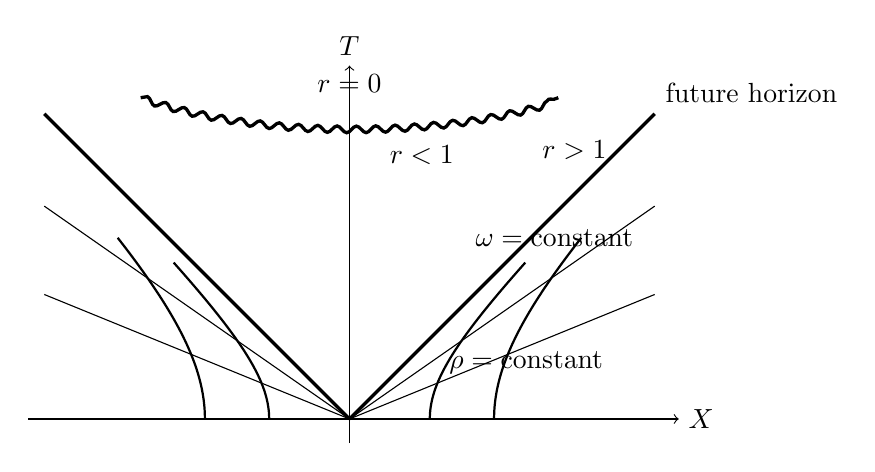
\begin{tikzpicture}[scale=1.02]
\draw[->] (-4.0,0) -- (4.1,0) node[right] {$X$};
\draw[->] (0,-0.3) -- (0,4.4) node[above] {$T$};
\draw[very thick] (0,0) -- (3.8,3.8)
  node[above right] {future horizon};
\draw[very thick] (0,0) -- (-3.8,3.8);
\draw[thick]
  plot[domain=0:1.42,samples=50]
  ({1.0*cosh(\x)},{1.0*sinh(\x)});
\draw[thick]
  plot[domain=0:1.05,samples=50]
  ({1.8*cosh(\x)},{1.8*sinh(\x)});
\draw[thick]
  plot[domain=0:1.42,samples=50]
  ({-1.0*cosh(\x)},{1.0*sinh(\x)});
\draw[thick]
  plot[domain=0:1.05,samples=50]
  ({-1.8*cosh(\x)},{1.8*sinh(\x)});
\draw[thin] (0,0) -- (3.8,1.55);
\draw[thin] (0,0) -- (3.8,2.65);
\draw[thin] (0,0) -- (-3.8,1.55);
\draw[thin] (0,0) -- (-3.8,2.65);
\draw[very thick,decorate,decoration={snake,amplitude=1.2pt,segment length=7pt}]
  (-2.6,4.0) .. controls (-1.2,3.5) and (1.2,3.5) .. (2.6,4.0);
\node at (0,4.18) {$r=0$};
\node at (2.2,0.7) {$\rho=\mathrm{constant}$};
\node at (2.55,2.25) {$\omega=\mathrm{constant}$};
\node at (0.9,3.28) {$r<1$};
\node at (2.8,3.35) {$r>1$};
\end{tikzpicture}
}
\caption{A clean causal reconstruction.  The horizon is a null line, while
the curvature singularity \(r=0\) is a future boundary inside the hole.}
\label{fig:l7-kruskal-clean}
\end{figure}

The small-\(\rho\) limit is unlike the small-radius limit in Euclidean polar
coordinates.  A small Euclidean circle contracts toward one point.  A
constant-\(\rho\) hyperbola approaches an entire null line.  Thus
\(\rho=0\) labels the whole horizon, not merely the crossing point of the
axes.

The exterior formula can be analytically continued to \(r<1\).  Near the
horizon, \(r-1\simeq\rho^2/4\), so the interior corresponds formally to
\(\rho^2<0\).  One may call \(\rho\) imaginary, but it is cleaner to use
\(\rho^2\), \(r\), or regular coordinates \(T,X\).  The signs of the
Schwarzschild \(t\) and \(r\) coefficients exchange inside.  That does not
mean that a physical wristwatch becomes a ruler.  It means the Schwarzschild
coordinates have exchanged their causal character.

\begin{classroomqa}
\audiencequestion{What are the horizontal hyperbolae inside the horizon, and
what are the straight rays?}
\lecturerresponse{The hyperbolic curves are constant \(r\), equivalently
constant \(\rho^2\), continued into \(r<1\).  The rays are constant
Schwarzschild time.  Outside they form a useful coordinate grid; inside the
same labels must not be mistaken for physical observer trajectories.
\lecturetimestamp{00:44:12--00:44:59}}
\end{classroomqa}

\begin{classroomqa}
\audiencequestion{Is the vertical direction a time coordinate, and whose
reference frame does it represent?}
\lecturerresponse{It is a regular time direction in the new spacetime
diagram, but it is not the singular Schwarzschild time \(t\).  The diagram is
adapted to freely falling causal structure.  An observer held at fixed
exterior radius follows a hyperbola and must accelerate; a freely falling
observer crosses the null horizon smoothly.
\lecturetimestamp{00:45:54--00:46:48}}
\end{classroomqa}

\begin{classroomqa}
\audiencequestion{If \(\rho^2<0\) inside, where is the explicit factor of
\(i\)?}
\lecturerresponse{One can introduce an imaginary \(\rho\), but nothing is
gained by doing so.  The invariant content is carried by \(r\), by
\(\rho^2\), and by the real regular coordinates \(T,X\).  The relation
\(r-1\simeq\rho^2/4\) is only the near-horizon expansion.
\lecturetimestamp{00:52:35--00:53:00}}
\end{classroomqa}

The regular diagram is often described in the lecture as the Kruskal
picture.  Strictly, the exact Kruskal coordinates include a radial factor
that keeps the full Schwarzschild metric regular, whereas
Eq.~\eqref{eq:l7-rindler-transform} is its near-horizon form.  The causal
message is the same: the horizon is smooth, but every future-directed
timelike or null curve inside ends at \(r=0\).  No superluminal turn can carry
it back through the horizon.

\subsection{How the Coordinate Singularity Was Understood}

The horizon's smoothness was historically difficult to see because the
original Schwarzschild coordinates make its coefficients look singular.
Eddington and later Finkelstein introduced coordinates that cross the
horizon, and Finkelstein recognized the one-way causal boundary.  Kruskal,
whose facility with coordinate changes came from plasma physics, supplied a
global regular picture of the eternal solution.

The lecture then pauses over John Wheeler, who helped make the phrase
"black hole" unavoidable.  The pause is personal as well as historical:
Wheeler is remembered as a gentle and thoughtful friend even where political
judgments, including judgments about nuclear competition, differed sharply.
A humorous personal anecdote is offered to resist a caricature of Wheeler as
socially conventional.  The technical point returns in the retort that
"black holes have no hair."  A disturbed nonrotating hole rapidly settles
toward spherical symmetry; a rotating one settles to the stationary shape
fixed by its conserved parameters.  This is the lecture's qualitative
version of the no-hair idea, not a proof of the full theorem.

\section{Alice Crosses; Bob Stays Outside}

The maximally extended diagram contains regions that do not occur in the
simple spacetime of a star collapsing from ordinary initial data.  For the
observer experiment we use only the exterior, the future horizon, and the
black-hole interior.

\begin{figure}[htbp]
\centering

\includegraphics[width=0.84\textwidth]{lecture_07_figure_04.png}
\caption{Alice's infalling worldline and the constant-Schwarzschild-time
rays.  The limiting ray is labelled \(t=\infty\).}
\lectureframe{00:54:54}
\end{figure}

Alice falls freely.  Her worldline crosses the horizon and reaches the
singularity in finite proper time.  Nothing singular happens to her clock at
the horizon if the black hole is large enough that tidal forces there are
small.

Bob instead remains at fixed exterior radius.  Holding station requires
acceleration.  Light from later points of Alice's trajectory reaches him
after increasing delays and with increasing redshift.  In Schwarzschild time,
Alice approaches \(t=\infty\) and Bob never receives a signal emitted after
her horizon crossing.  These are statements about causal signals and the
outside slicing, not evidence for a material surface at the horizon.

\begin{classroomqa}
\audiencequestion{If Bob sees Alice slow down, must Alice see Bob speed up?}
\lecturerresponse{No.  Alice continues to receive ordinary light signals
from Bob while her worldline lasts.  There is a last event on Bob's worldline
that can reach her, but that event is last only because Alice subsequently
hits the singularity.  Nothing abrupt happens to Bob.  Observation always
looks into a past light cone, and the two worldlines have an asymmetric
causal relation.
\lecturetimestamp{00:58:31--01:01:23}}
\end{classroomqa}

\begin{classroomqa}
\audiencequestion{If Bob knows that Alice is still close to the horizon in
his coordinates, can he go down, retrieve her, and return?}
\lecturerresponse{A rescue worldline must meet Alice before she crosses the
event horizon.  After that event no future-directed path can meet her and
return outside.  The fact that Schwarzschild slices place the crossing at
\(t=\infty\) does not leave Alice sitting on a retrievable material surface;
it shows that those slices do not provide a global notion of "now" across
the horizon.
\lecturetimestamp{01:01:24--01:02:12}}
\end{classroomqa}

\section{Charlie Follows Alice}

Let Charlie fall a short distance behind Alice.  Both are then approximately
inertial near the horizon.  They can exchange signals, converse in both
directions, or even hold hands.  Neither finds a signpost marking the horizon.
The contrast with Bob is not a contrast between three named people.  It is a
contrast between free fall and an accelerated worldline that remains outside.

\begin{classroomqa}
\audiencequestion{What does Bob see if Alice falls first and Charlie follows,
like a basketball following a hoop?}
\lecturerresponse{Bob sees both approach the horizon.  Alice, being ahead,
appears progressively slowed and radially compressed first.  Charlie appears
closer and closer behind her but never catches her in Bob's limiting outside
view.  The visual piling-up does not describe what either infaller feels.
\lecturetimestamp{01:04:12--01:06:05}}
\end{classroomqa}

\begin{classroomqa}
\audiencequestion{Does the apparent flattening contradict the tidal force,
which should stretch an infaller radially?}
\lecturerresponse{They are different effects.  The flattening belongs to
Bob's Schwarzschild-coordinate description.  Tidal elongation is a local
curvature effect that Alice and Charlie can feel.  The observer discussion
assumes a sufficiently large black hole, or sufficiently small observers, so
that the tidal effect at the horizon is negligible.  A roughly solar-mass
hole would instead have fierce horizon tides, while a supermassive one can
have weak horizon tides.
\lecturetimestamp{01:06:07--01:08:18}}
\end{classroomqa}

\begin{classroomqa}
\audiencequestion{Does Charlie see Alice cross while he is still outside?}
\lecturerresponse{Draw the null ray.  The light emitted at Alice's crossing
runs along the horizon and reaches Charlie when Charlie crosses.  At that
event he can calculate that he has seen her crossing, although neither
observer encounters a local marker.  Afterward he can see her inside.  If he
accelerates away before crossing and succeeds in remaining outside, he never
sees the crossing.
\lecturetimestamp{01:08:19--01:11:11}}
\end{classroomqa}

\begin{classroomqa}
\audiencequestion{If Alice is already inside while Charlie is outside, how
can their later radii and crossing times be compared?}
\lecturerresponse{There is no observer-independent simultaneity relation to
read off from a phrase such as "at the same time."  Alice sees Charlie on her
past light cone and can see his later crossing only when she is farther
inside.  The specific worldlines and null rays answer the question.  A broad
extrapolation to many widely separated infallers must be checked by drawing
their actual causal diagram rather than assuming one universal crossing time.
\lecturetimestamp{01:11:14--01:12:31}}
\end{classroomqa}

In the regular near-horizon coordinates, a free-fall trajectory is nearly a
straight line.  It is not exactly straight in the full Schwarzschild
geometry, but the approximation becomes good near a large, weakly curved
horizon.

\begin{classroomqa}
\audiencequestion{Can string theory settle what happens in the
quantum-gravity regime of the black-hole interior?}
\lecturerresponse{That is precisely where the subject becomes subtle.  A
quantum theory of gravity is required near the singularity, and string theory
is a candidate framework, but the relevant questions were active and
difficult rather than solved by a simple application of the classical
diagram.
\lecturetimestamp{01:13:04--01:13:38}}
\end{classroomqa}

\begin{classroomqa}
\audiencequestion{What happens to Alice's own clock and velocity as she
crosses?}
\lecturerresponse{Her clock keeps ticking at its ordinary local rate and
records finite proper time.  In her instantaneous rest frame she is at rest;
relative to a local freely falling frame she has an ordinary finite velocity.
Near a large horizon the geometry is almost flat, so equal proper-time marks
along her worldline remain regular until curvature becomes strong near the
singularity.
\lecturetimestamp{01:13:39--01:14:44}}
\end{classroomqa}

\begin{classroomqa}
\audiencequestion{What if Bob accelerates outward but not quite hard enough
to avoid falling through?}
\lecturerresponse{Then his worldline bends outward but still crosses the
horizon.  If he crosses very late, he can see Alice shortly after her
crossing, but his remaining proper time before the singularity is short.
Worldline slopes on the sketch are not calibrated rulers or clocks; the
causal ordering, not their drawn Euclidean lengths, is what survives.
\lecturetimestamp{01:14:47--01:16:31}}
\end{classroomqa}

All of these conclusions assume that no signal outruns light.  The lecture
briefly jokes about then-recent press reports of apparently superluminal
neutrinos in Italy, an allusion to an experimental timing error rather than
an exception to relativity.  The causal construction itself remains bounded
by the null lines.

\begin{classroomqa}
\audiencequestion{Can synchronized clocks carried by Alice and Bob decide
the issue if Alice dives toward the horizon and returns?}
\lecturerresponse{They may compare clocks when they coincide, but after their
worldlines separate there is no unique distant synchronization, especially
when one changes motion.  Draw both worldlines and the exchanged null rays.
That diagram supplies the operational answer to any specified experiment.
\lecturetimestamp{01:17:34--01:18:25}}
\end{classroomqa}

\begin{figure}[htbp]
\centering

\includegraphics[width=0.86\textwidth]{lecture_07_figure_05.png}
\caption{The accumulated causal diagram used to answer the Alice, Bob, and
Charlie questions.  Each observation is located by tracing a null ray from
the observed event to the observer's worldline.}
\lectureframe{01:18:12}
\end{figure}

\begin{figure}[htbp]
\centering
\resizebox{0.96\linewidth}{!}{%
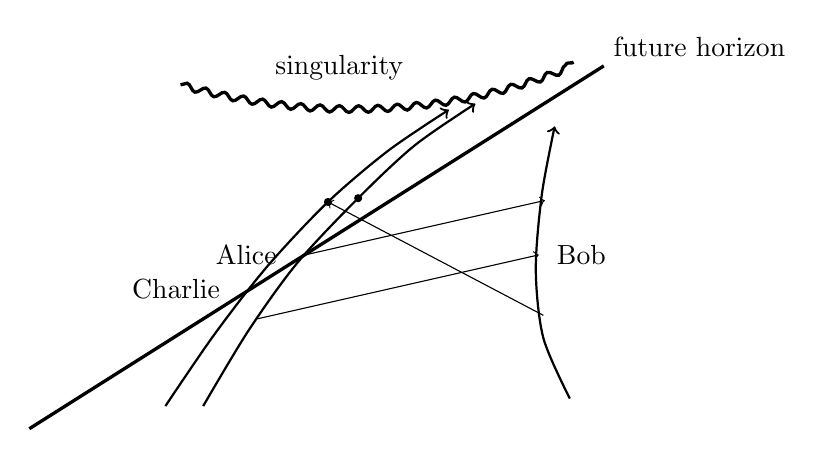
\begin{tikzpicture}[scale=0.96]
\draw[very thick] (-3.8,-0.3) -- (3.8,4.5);
\node[above right] at (3.8,4.5) {future horizon};
\draw[very thick,decorate,decoration={snake,amplitude=1.2pt,segment length=7pt}]
  (-1.8,4.25) .. controls (0.1,3.72) and (2.0,3.92) .. (3.4,4.55);
\node at (0.3,4.48) {singularity};
\draw[thick,->]
  plot[smooth] coordinates {(-1.5,0.0) (-0.9,1.0) (-0.25,1.9)
  (0.55,2.75) (1.3,3.45) (2.1,4.0)};
\node[left] at (-0.4,2.0) {Alice};
\draw[thick,->]
  plot[smooth] coordinates {(-2.0,0.0) (-1.35,0.95) (-0.65,1.85)
  (0.15,2.7) (0.95,3.38) (1.75,3.92)};
\node[left] at (-1.15,1.55) {Charlie};
\draw[thick,->]
  plot[smooth] coordinates {(3.35,0.1) (3.0,0.9) (2.9,1.8)
  (2.98,2.8) (3.15,3.7)};
\node[right] at (3.05,2.0) {Bob};
\draw[thin,->] (-0.8,1.15) -- (2.94,2.0);
\draw[thin,->] (-0.15,2.0) -- (3.02,2.72);
\draw[thin,->] (3.0,1.2) -- (0.15,2.7);
\draw[fill] (0.55,2.75) circle (1.3pt);
\draw[fill] (0.15,2.7) circle (1.3pt);
\end{tikzpicture}
}
\caption{A schematic observer diagram.  Bob's exterior observations and the
mutual observations of Alice and Charlie are different null-ray
constructions, not reciprocal clock slogans.}
\label{fig:l7-observers-clean}
\end{figure}

\begin{classroomqa}
\audiencequestion{Does Bob see Alice for an infinite time, and does that mean
she never dies in his reality?}
\lecturerresponse{Bob receives her signals over an unbounded interval of his
time, but he sees her clock slow toward zero rate and receives only the
finite sequence of heartbeats emitted before her crossing.  The word
"reality" hides the distinction between a local event and an observer's
asymptotic record.  Alice experiences no stopped clock at the horizon; Bob's
record is increasingly delayed and redshifted.
\lecturetimestamp{01:18:32--01:20:59}}
\end{classroomqa}

\begin{classroomqa}
\audiencequestion{Does Alice suddenly see all the old matter that appeared
frozen on the horizon once she crosses?}
\lecturerresponse{No sudden clearing occurs.  As she falls, the past light
cones by which she sees earlier matter change continuously.  She can infer
that light reaching her now was emitted earlier and that the matter crossed
before her.  Charlie's view of Alice supplies the same lesson: neither
crossing produces a local discontinuity or reveals a hidden pile of chairs
and dinosaurs.
\lecturetimestamp{01:21:02--01:23:48}}
\end{classroomqa}

\begin{classroomqa}
\audiencequestion{Are there realistic simulations of what an infaller would
see?}
\lecturerresponse{The lecture points to Andrew Hamilton's black-hole
visualizations.  They can convey the severe aberration and frequency shifts
of incoming light, although the display may be more disorienting than
illuminating.  "Nothing special at the horizon" refers to local geometry, not
to an ordinary-looking sky.
\lecturetimestamp{01:24:11--01:25:29}}
\end{classroomqa}

\section{From an Eternal Hole to a Growing Hole}

The lower apex of the maximally extended eternal diagram has little direct
significance for a black hole formed by stellar collapse.  Only the portion
containing the exterior, the future horizon, and the future interior appears
in the simple collapse geometry.  This distinction becomes essential when
matter is allowed to change the mass of the hole.

\begin{classroomqa}
\audiencequestion{What physical event is represented by the lower apex of
the idealized diagram?}
\lecturerresponse{For the eternal mathematical solution it is part of the
maximal extension.  A black hole formed from collapsing matter does not
contain that whole lower region.  Its horizon has a formation history, which
requires a different global diagram and is developed in the next lecture.
\lecturetimestamp{01:25:59--01:26:52}}
\end{classroomqa}

When a small test body falls in, its backreaction can be neglected and the
fixed Schwarzschild diagram is adequate.  If a substantial mass falls in,
the black-hole mass and Schwarzschild radius increase:
\begin{equation}
r_{\mathrm S}=2GM,
\qquad
\Delta r_{\mathrm S}=2G\,\Delta M.
\label{eq:l7-growing-radius}
\end{equation}
The horizon deforms toward the incoming object, the horizons join, and the
distorted common horizon rapidly settles.  In the lecture's nonrotating
idealization the endpoint is a slightly larger sphere.  A real merger also
radiates energy in gravitational waves and generally leaves a rotating hole.

\begin{classroomqa}
\audiencequestion{If the horizon grows when mass falls in, does it move
outward to meet matter that seemed frozen near the old horizon?}
\lecturerresponse{For a sufficiently massive infalling object the
test-particle picture is no longer valid.  The horizon deforms, joins the
incoming object's trapped region, and relaxes to a larger stationary
horizon.  The exact placement of the event horizon is global and can extend
into a region before the infalling matter arrives.  The lecture deliberately
defers the full construction to the next meeting.
\lecturetimestamp{01:26:55--01:29:05}}
\end{classroomqa}

\begin{classroomqa}
\audiencequestion{Why can astronomers see flashes when matter is said to take
infinite Schwarzschild time to reach the horizon?}
\lecturerresponse{The bright radiation does not come from the horizon
itself.  Gas in an accretion flow or disk collides and heats outside the
horizon, including near strong photon orbits.  That exterior plasma can emit
light that reaches us.  The empty Schwarzschild geometry isolates the causal
problem but is not a complete model of an astrophysical environment.
\lecturetimestamp{01:29:07--01:30:22}}
\end{classroomqa}

The characteristic relaxation time is set by the light-crossing time:
\begin{equation}
t_{\mathrm{cross}}\sim\frac{r_{\mathrm S}}{c},
\qquad
t_{\mathrm{relax}}\sim
\text{a few to a few tens of }t_{\mathrm{cross}}.
\label{eq:l7-relaxation-scale}
\end{equation}
The lecture estimates \(10^{-5}\,\mathrm{s}\) as the crossing time of a
kilometer-scale hole and roughly \(10^{-3}\,\mathrm{s}\) for a small merger
to become nearly stationary.  For a billion-solar-mass hole the corresponding
time is measured in minutes to hours.  These are scaling estimates, not
precision merger calculations.  The geometric sequence is the point:
dumbbell, peanut, nearly spherical, stationary.

\begin{classroomqa}
\audiencequestion{How fast does a distorted or newly merged horizon settle?}
\lecturerresponse{On a time scale not vastly longer than light needs to cross
the hole.  Because every length and time scales with \(r_{\mathrm S}\), small
holes settle in fractions of a second and supermassive holes on much longer
clock times.  The no-hair statement describes the stationary endpoint; the
transient deformation carries away energy through gravitational radiation.
\lecturetimestamp{01:30:26--01:33:18}}
\end{classroomqa}

\begin{classroomqa}
\audiencequestion{What does Bob see if earlier matter lies between the old
and new horizon while another heavy body falls in?}
\lecturerresponse{That question cannot be answered consistently by patching
two static Schwarzschild diagrams together.  One must solve or construct the
time-dependent collapse geometry and locate its global horizon.  The lecture
keeps the question and explicitly postpones the answer to the next week,
where horizon formation is the subject.
\lecturetimestamp{01:33:20--01:35:41}}
\end{classroomqa}

\section{What Changes When the Scale Changes?}

The dimensionless diagram does not change when \(r_{\mathrm S}\) changes.
The physical meaning of a drawn interval does:
\begin{equation}
d\tau_{\mathrm{physical}}^2
=
r_{\mathrm S}^2\,d\hat{\tau}^2,
\qquad
\ell_{\mathrm{physical}}
=
r_{\mathrm S}\,\hat{\ell}.
\label{eq:l7-scale-restoration}
\end{equation}
A dimensionless separation that represents half a kilometer for a
kilometer-scale hole represents roughly half a billion kilometers for a hole
a billion times larger.  The analogy with equally drawn spheres returns: the
shape is unchanged, while the number of meter sticks represented by a line
scales with the radius.

\begin{classroomqa}
\audiencequestion{How does the causal diagram change as the Schwarzschild
radius changes?}
\lecturerresponse{It does not change after the radius has been scaled out.
Every physical length and time assigned to the diagram is multiplied by
\(r_{\mathrm S}\), while curvature at corresponding dimensionless points is
multiplied by \(r_{\mathrm S}^{-2}\).
\lecturetimestamp{01:35:41--01:38:10}}
\end{classroomqa}

\begin{classroomqa}
\audiencequestion{Does the causal conclusion change if Bob orbits instead of
hovering at one angular position?}
\lecturerresponse{The detailed redshifts and arrival directions become more
complicated, but the horizon's causal separation does not change.  No
exterior timelike orbit receives a signal emitted from inside the horizon.
\lecturetimestamp{01:38:12--01:38:26}}
\end{classroomqa}

\begin{classroomqa}
\audiencequestion{Since gravity vanishes inside a spherical shell, does it
vanish inside the horizon because the black-hole mass is spread over that
surface?}
\lecturerresponse{No.  The event horizon is not a material shell carrying
the mass.  The Newtonian shell theorem therefore does not apply to it.  The
lecture compares the static exterior solution to a point source at the
curvature singularity, but matter currently falling during formation
requires the time-dependent geometry deferred to the next lecture.
\lecturetimestamp{01:38:28--01:40:41}}
\end{classroomqa}

\section{Rotation and Radial Geometry}

Angular momentum survives collapse.  A rotating black hole has an exterior
geometry different from Schwarzschild: its stationary solution is Kerr,
rotation distorts the horizon geometry, and frame dragging carries inertial
directions around the hole.  In principle the angular momentum is measured
from those exterior gravitational effects.  Matter with angular momentum
does not lose it merely by crossing a horizon.

\begin{classroomqa}
\audiencequestion{Can a black hole have measurable angular momentum, and
does rotation change gravity outside it?}
\lecturerresponse{Yes.  The angular momentum remains as a conserved
parameter, deforms the stationary geometry, and produces frame dragging.
The horizon is no longer the simple spherical Schwarzschild horizon.  The
lecture compares the distortion qualitatively with the Earth's oblate shape,
while noting that the full rotating solution is substantially more
complicated.
\lecturetimestamp{01:40:45--01:42:36}}
\end{classroomqa}

\begin{classroomqa}
\audiencequestion{Does the relation between \(r\) and proper distance
\(\rho\) mean that gravity contracts space?}
\lecturerresponse{The proper radial distance \(\rho\) satisfies
\begin{equation*}
\frac{d\rho}{dr}=\sqrt{\frac{r}{r-1}}>1
\end{equation*}
outside the unit horizon. A given coordinate increment \(dr\) therefore
corresponds to a larger proper radial interval near the horizon. Saying that
space is contracted or stretched depends on which coordinate intervals are
being compared. The invariant statement is the proper-distance relation
itself.
\lecturetimestamp{01:42:36--01:43:20}}
\end{classroomqa}

\section{Final Questions}

\begin{classroomqa}
\audiencequestion{From Bob's view Alice's clock approaches a stop.  From
Alice's view, does Bob's space or time come to an end?}
\lecturerresponse{No.  Alice sees ordinary signals from successive events on
Bob's worldline until her own worldline ends.  She fails to see later Bob
events because no later point on her worldline exists, not because Bob or his
space disappears.  In these regular causal coordinates radial null rays are
drawn straight; their appearance as curved paths in another coordinate
system does not alter which events they connect.
\lecturetimestamp{01:43:21--01:45:20}}
\end{classroomqa}

General relativity presents two complementary tasks.  Given a metric, one can
trace geodesics and null rays to determine what observers measure.  Given a
distribution of matter, one must solve Einstein's equations to find the
metric.  The first task has occupied this lecture.  The second is usually
harder, although symmetric collapse provides tractable examples.

\begin{classroomqa}
\audiencequestion{What happens to the horizon and singularity of an
evaporating black hole?}
\lecturerresponse{The lecture gives a schematic picture in which the horizon
shrinks and meets the endpoint of the singular region.  Evaporation is a
semiclassical quantum process, and the final Planck-scale endpoint is not
settled by the classical Schwarzschild diagram.  The shrinking sketch should
therefore be read as a qualitative preview, not a complete quantum geometry.
\lecturetimestamp{01:46:04--01:46:32}}
\end{classroomqa}

Almost every astrophysical black hole should rotate.  Stars already possess
angular momentum, and collapse amplifies their angular velocity in the
familiar manner of a skater drawing in their arms.  The singular structure of
a Kerr black hole is not the Schwarzschild \(r=0\) surface drawn here, and it
should not be described as matter literally rotating with infinite linear
speed.

\begin{classroomqa}
\audiencequestion{Are nonrotating macroscopic black holes common, and how
many black holes are there?}
\lecturerresponse{Exactly zero angular momentum would be an exceptional
idealization.  The lecture gives only an order-of-magnitude classroom guess
for the cosmic population, somewhere between galaxy and stellar counts and
perhaps around \(10^{15}\).  That is a lecture-era estimate, not a measured
census.  The robust point is that collapse generically preserves and
amplifies some angular momentum.
\lecturetimestamp{01:46:32--01:48:42}}
\end{classroomqa}

\begin{classroomqa}
\audiencequestion{Do black holes form from existing matter or appear through
a quantum process?}
\lecturerresponse{Ordinary astrophysical holes form when existing stellar
matter collapses.  Nuclear burning and the outward flow of energy help
support a star.  When fuel is exhausted, the remnant contracts.  Depending
on its mass and available pressure support, it may become a white dwarf, a
neutron star, or, if no support can halt collapse, pass within its own
Schwarzschild radius and form a black hole.
\lecturetimestamp{01:48:43--01:50:23}}
\end{classroomqa}

\begin{classroomqa}
\audiencequestion{Could microscopic black holes form, and what would set
their lifetime and minimum size?}
\lecturerresponse{This part is speculative.  Hawking evaporation is faster
for smaller mass, with a lifetime that scales approximately as \(M^3\).
The lecture uses a mountain-mass comparison for a hole whose lifetime might
be cosmological; the numerical analogy is only rough.  Violent density
fluctuations in the early universe or sufficiently energetic collisions are
conceivable formation mechanisms.  A black hole near the Planck mass,
roughly \(10^{-5}\,\mathrm{g}\), marks the scale where a classical geometric
description ceases to be trustworthy.  Reaching that energy in an ordinary
accelerator would require an implausibly large machine under straightforward
extrapolation, although the formation statement is possible in principle.
\lecturetimestamp{01:50:23--01:53:31}}
\end{classroomqa}

\begin{classroomqa}
\audiencequestion{Will the course reach cosmology, dark matter, dark energy,
entropy, and gravitational waves?}
\lecturerresponse{Cosmological applications and perhaps gravitational waves
remain possible later topics.  Black-hole entropy is deferred beyond the
quarter.  The lecture closes by accepting that only about a quarter of the
planned material was covered that evening: resolving the questions carefully
matters more than racing through the outline.
\lecturetimestamp{01:53:33--01:54:38}}
\end{classroomqa}

The operational rule survives every question in the room.  Specify the
worldlines, draw the null rays, and locate the events they connect.  The
horizon is not a place where local physics breaks; it is the boundary beyond
which every future-directed signal remains inside.  The next lecture replaces
the eternal background by a collapsing source and shows how that boundary is
formed.
